\documentclass[11pt,letter,oneside]{report}
\usepackage[pdftex]{graphicx}
\usepackage{float}
\begin{document}

\title{Space Invaders}
\author{Peter Hamilton and Jared Pilcher}
\date{Fall 2011}
\maketitle

\tableofcontents

\chapter{Space Invaders Overview}
\section{History of Space Invaders}

Designed by Tomohiro Nishikado in 1978, Space Invaders is one of the greatest arcade games of all time. It took Nishikado over a year to develope the game and its hardware. It was manufactured in Japan by Taito. It was so influential that it pushed the video game industry into a worldwide industry. Shortly after its release, it caused a shortage of 100-yen in Japan. By 2007, Taito earned over \$500 million dollars in profits. 

Space invaders was a really popular game in 1978. It is one of the most influential and successful games of all time. It is a two dimensional shooting game involving a tank that shoots aliens marching across a screen. When all of the aliens were destroyed, or all of the lives of the tank were used, the game ended. It has had several sequels, and was released on several platforms. It was the inspiration for many other video games on the market today. 

To this day, a bug still exists from the original game. In the original game, as the marching aliens were killed, the game refreshed faster since there was less to load an the screen. This added an extra challenge to the game. As the game became popular, consumers became accustomed to the bug. When the developer fixed the bug, the market responded poorly. It was placed back into the game, and has been there since.
 
\section{Game Play}

\subsection{Objective}

The world is being invaded by marching aliens.  All of humanity has gathered behind 4 bunkers for protection.  You control the only weapons available, a supply of 3 tanks and a handful of missiles. Kill all the aliens! Watch out! The alien mothership flies over head! Destroy it at all costs!  The fate of the world rests in your hands...

Win the game by killing all of the marching aliens. Destroying the mothership gives you extra points.

\subsection{The Tank}
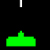
\includegraphics[]{tank.jpg}

You are the tank. Push the left button to move left, and the right button to move right. You can fire and move simultaneously.

Watch out! Enemy fire rains from above! Dodge the alien fire by moving the tank left or right. Each time your tank is hit by an alien bullet, it explodes. You have three lives.  You must survive...

Fire your missile to destroy the alien invaders! Push the middle button to fire your missile, aiming for the aliens. When the missile hits an alien, it dies. Be careful! They move left and right, and get closer as time goes on.

\subsection{Enemies}

\subsubsection{Spaceship}

\includegraphics[]{big-alien.png}

The alien mothership circles the Earth, looking for its prey. Destroy it at all costs! It flies occasionally from left to right. As it flies overhead, launch your tank missile by pushing the middle button. Be careful, it tries to evade you missile, so shoot accurately and quick!


\subsubsection{Aliens}

\includegraphics[]{aliens.jpg}

55 aliens are marching toward your position! You are charged with destroying all of them before they reach you! Fire your missiles to kill them! These aliens can shoot up to four bullets at a time. 

Aliens are capable of destroying walls, so your bunkers will provide no protection when they reach them. Their bullets slowly degrade your bunkers when they're hit. Be quick! You will soon have no protection!

\subsection{Points}
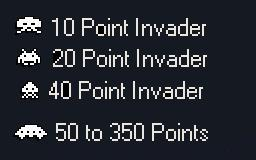
\includegraphics[]{scoring.jpg}

Earn points by destroying the aliens with your tank missiles. The lower two rows of aliens, middle two rows of aliens, and the top row of aliens are worth 10, 20 points and 40 points per alien, respectively.

Earn extra points for destroying the mothership! Earn between 50 to 350 points for each mothership destroyed.

\section{Game Details and Specifications}

\subsection{Aliens}

\subsubsection{Alien Placement and Appearance}
There are 55 aliens that start on the screen.  They are on a 11 by 5 grid.  Each grid is 15 pixels by 15 pixels.  There are three types of aliens.  The first two rows are the widest aliens, the next two rows are a little narrower and the top row has the narrowest alien.

\subsubsection{Alien Movement}
The aliens move laterally in increments of 2 pixels.  When the rightmost aliens reach the right edge of the screen, the grid of aliens will move down 7 pixels and start moving left.  When the leftmost aliens reach the left edge of the screen, they will move down 7 pixels and start moving right.  The rightmost alien and leftmost alien is the closest alien to the respective sides that has not been killed. This means that when the rightmost column of aliens are destroyed, the aliens march toward the side of the screen until the next column hits that side. The aliens continue this pattern of movement until the bottommost row of alive aliens reaches the bottom of the bunkers. The aliens will speed up in their movement as aliens are killed.

\subsubsection{Alien Explosions}
When an alien is hit by a bullet from the tank, it blows up.  The other aliens continue onward while the explosion sequence is happening.

\subsection{Alien Mothership}
The alien mothership flies across the screen from left to right. It's time of appearance is random. When a bullet strikes the mothership, it flashes, revealing the score received.

\subsection{The Tank}
\subsubsection{Movement}
The tank moves laterally across the bottom of the screen. The user is able to push the right button to move right, or push the left button to move left at a rate of two pixels. The user is able to hold down the left or right buttons to keep the tank moving across the screen.
\subsubsection{Firing Bullets}
You may also fire a missile by pushing the middle button. The tank is capable of moving and firing simultaneously. It is also capable of changing direction while shooting. This means that you are able to hold down the fire button and change directions.
\subsubsection{Death}
When the tank is struck by an alien bullet, it explodes.  The player will lose a life and continue the current level.

\subsection{Bullets}
\subsubsection{Tank Bullets}
Tanks are capable of firing bullets by pushing the middle button. Tank bullets, unlike Alien Bullets, only have one appearance. They are white rectangles that are ejected just above the center of the tank. No black boxes surround the bullet. In other words, when it leaves the tank, or strikes an object, an overlay of a black box cannot be seen. 

When a bullet is on the screen, the tank cannot fire again until the bullet has left the screen. Each bullet travels at a rate of 2 pixels. When it strikes an alien or mothership, the object is destroyed.

\subsubsection{Alien Bullets}
There are two types of alien bullets:
\begin{enumerate}
\item{}  Zig zag bullets rotate cyclically through the following appearances:

\begin{enumerate}
\item 
 
\includegraphics[scale=2]{ZigBullet0.png}
\item 
 
\includegraphics[scale=2]{ZigBullet1.png}
\item
 
\includegraphics[scale=2]{ZigBullet2.png}
\item
 
\includegraphics[scale=2]{ZigBullet3.png}
\end{enumerate}

\item{}  Cross bullets oscillate through the following appearance:

\begin{enumerate}
\item
 
\includegraphics[scale=2]{TBullet0.png}
\item
 
\includegraphics[scale=2]{TBullet1.png}
\item
 
\includegraphics[scale=2]{TBullet2.png}
\end{enumerate}

\end{enumerate}

Each bullet is ejected from the center of an alien, randomly chosen to be an alien on the bottommost row. There can only be 4 bullets on the screen at any given point in time.  Once a bullet leaves the screen, a new bullet can be fired. Each bullet travels at a rate of 2 pixels. When the bullet strikes a tank, it is destroyed. When the bullet strikes a bunker, the bunker is eroded. When a piece of the bunker is completely eroded, the bullet can pass through it.  No black boxes surround the bullet. In other words, when it leaves an alien, or strikes an object, an overlay of a black box cannot be seen. 

\subsection{The Bunkers}
There are four bunkers available for the tank to use as cover.  Each bunker is divided into 10 sections.  Each section partially erodes with each collision of an alien bullet.  After 4 collisions, the section is fully eroded and will allow bullets to pass through.

When the aliens reach the bunkers, they will walk above the bunkers as they move through them. In other words, they will be drawn over the bunkers and those portions of the bunkers will be destroyed.


\subsection{Scoring}
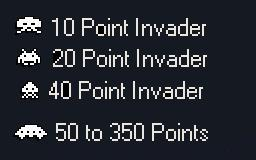
\includegraphics[]{scoring.jpg}

Earn points by destroying the aliens with your tank missiles. The lower two rows of aliens, middle two rows of aliens, and the top row of aliens are worth 10, 20 points and 40 points per alien, respectively.

\subsection{End of Game}
The game ends when one of the following three events occur:
\begin{enumerate}
\item The bottommost row of aliens that are alive reach the bottom of the bunkers.
\item The tank has been destroyed three times.
\item All aliens are destroyed.
\end{enumerate}
When the game ends, a game over screen is displayed.

\subsection{Appearance}
The game appearance is identical to the flash version of Space Invasion. The game runs smoothly and at a decent speed. The screen is also updated close to the same rate as the flash-based game. No artifacts appear on the screen. No flickering occurs on the screen.

\chapter{Game Console and Engine}

\section{Game Console}
\subsection{Xilinx University Program Board}
	\subsubsection{Virtex II Pro}
		The board we are using contains a Virtex II Pro XC2VP30. The specifications are as follows:
		\begin{itemize}
			\item 2 PowerPC Processor Blocks
			\item 30,816 Logic Cells
			\item 13,696 Slices for a maximum of 428 Kb of Distributed RAM
			\item 136 18 x 18 bit multiplier blocks
			\item 136 18Kb Blocks of SelectRAM+ for a maximum RAM block of 2,448 Kb
			\item 8 DCMs
			\item A Maximum of 644 User I/O Pads
		\end{itemize}
   	\subsubsection{256 DDR Memory}
		The 256MB DDR Memory provides additional memory for the program to use.    The board can use either buffered or unbuffered memory with a maximum capacity of 2 GB.  The RAM is Double Data Rate, which allows for faster reads and writes than are typical with SDRAM.  It achieves double the data rate by reading and writing on both the rising and falling edges of the clock cycle.  Even with the Double Data Rate, reads and writes to the DRAM are quite slow in comparison to local cache and should be avoided in performance critical applications.
	\subsubsection{AC-97 Sound Controller and jacks}
		The AC-97 Sound Controller resides on the FPGA board acts as a buffer and encoder for the AC-97 hardware. The AC-97 hardware is only able to accept serial data. To make the driver programming easier, the Sound Controller hardware accepts a large quantity of 32 bit words and sends it to the AC-97 hardware in a serial data stream. Furthermore, it sends the data to an Analog Codec and sends the stream to the the AC-97 hardware. Lastly, the analog codec receives analog signals through a MIC\_IN port and translates it to a serial digital signal. The AC-97 port transforms this data into 32 bit words and sends them to the PPC.
		\begin{itemize}
		\item LINE\_IN

		The input signal line from the LINE\_IN port on the board. It is not amplified, but it is filtered by the Analog Codec and digitized.
		\item LINE\_OUT

		The signal line that is sent to the amplified PC speaker array through a jack port.
		\item MIC\_IN

		The input signal line from the MIC\_IN port on the board. It is later amplified and filtered by the Analog Codec and digitized.
		\item AMP\_OUT
		
		The amplified signal line that is sent to the headphone jack for listening.
		\end{itemize}
		\begin{figure}[ht]
		\centering
		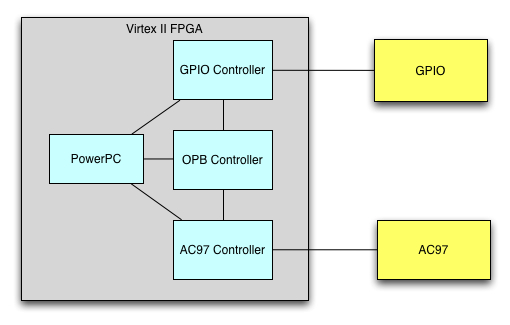
\includegraphics[scale=.8]{AC97.jpg}
		\caption{AC-97 controller overview. The AC-97 Controller acts as a buffer to the AC-97 hardware.}
		\label{fig:ac97}
		\end{figure}
     	\subsubsection{VGA Controller}
		The VGA controller actively draws the contents of a frame buffers to the screen. The frame buffer is defined by a range of memory addresses on the DDR. The user specifies the address of the frame buffer. The vga controller is a block of IP placed in the FPGA fabric. The Video DAC converts 8 bits per color (24 bits per pixel) to the corresponding analog signal for the output to the VGA.

		\begin{figure}[ht]
		\centering
		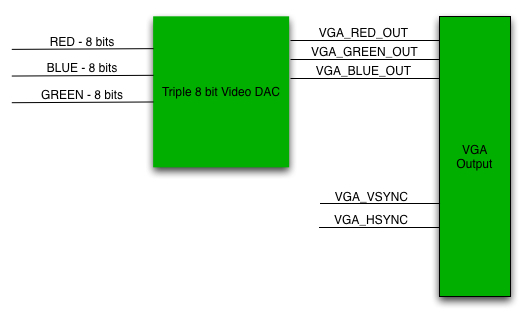
\includegraphics[scale=.8]{VGA.jpg}
		\caption{VGA controller. Three 8 bit signals are sent to the DAC, which transforms it into an analog signal in red, green and blue.}
		\label{fig:vga}
		\end{figure}
	\subsubsection{Compact Flash}
		Compact Flash provides non volatile memory that allows data to be persistent across resets. The FPGA logic can be stored on this memory to provide support for board resets. Upon resetting, the logic is loaded from the flash memory into the FPGA board if configured to do so.
	\subsubsection{UART/JTAG for debugging purposes}
	\label{sec:jtag}
		The Xilinx stdio library provides access to the UART.  Input and output operations that would normally be to STDOUT and from STDIN are instead made to the UART.  Print statements can be read via the UART on a connected machine,  and input from the connected machine can be read by the stdio library via the UART.  JTAG provides a method of programming the FPGA and/or the system memory.  JTAG on the board can use 3 different sources to program the board.  It can use the Compact Flash at boot time.  It can use a USB to PC connection.  It can use a PC4 cable connection.  Each of these methods is advantageous in different scenarios, and the priority is specified via switches on the board.

\subsection{Xilinx Virtex II. Pro EDK System}
	\begin{itemize}
		\item \textbf{PowerPC 405:}
			There are 2 PowerPC 405 cores in the FPGA.  They can be disabled but they cannot be reconfigured.  They operate at 300 Mhz.  They interact with various components through the OPB Bus, such as the GPIO Controller, the AC-97 Controller.  It can interact with other components (such as SATA or Ethernet) via the OPB Bus.  It interacts directly with the interrupt controller.
		\item \textbf{OPB:}
			The On-Chip Peripheral Bus is a data bus between peripheral controllers.  The OPB bus controller handles the how this bus is accessed.
		\item \textbf{AC-97 Controller:}
			See Figure~\ref{fig:ac97}.  The AC-97 controller buffers output to the AC-97 hardware.  Other controllers and the PowerPC interact with it via the OPB.  It is not a reconfigurable component of the FPGA.
		\item \textbf{GPIO Controller:}
			The GPIO Controller handles input and output to the GPIO modules (such as LEDs, switches, and push buttons).  It interacts with other controllers and the PowerPC via the OPB.  It is not a reconfigurable component of the FPGA.
		\item \textbf{VGA Controller:}
			The VGA Controller includes a video DAC and the IP necessary to drive the sync signals of a VGA output.  It is not a reconfigurable component.  It interacts with the system via the OPB.  It connects to the VGA output port on the board.
		\item \textbf{UART:}
			The UART handles communication via the RS-232 port on the board.  This is configurable logic and many UART IPs exists which can be used with the board.
		\item \textbf{Ethernet:}
			The ethernet port on the board is the PHY layer of the ethernet protocol. This allows high speed network capabilities. The Ethernet controller is configurable logic.  The EDK ships with many different ethernet modules that can be used.
		\item \textbf{Multi-gigabit Transceiver:}
			The FPGA has 8 multi-gigabit Transceivers.  3 of these are accessible via the SATA ports.  The Multi-gigabit Transceiver is not configurable logic, but additional logic would be necessary to implement the SATA protocol above the PHY layer.  The board provides a 75Mhz clock in order to use the transceivers.
		\item \textbf{SDRAM memory controllers:}
			The board has a DDR memory slot.  The The controller for the memory is configurable logic and there are many controllers to choose from.  The memory controller interacts with various parts of the system.  The PowerPC core has a MMU which communicates with the memory controller.
		\item \textbf{High Speed Expansion Port:}
			The board has a high speed expansion port.  Any implementation of a high speed protocol must be done in reconfigurable logic.
		\item \textbf{CPU Debug Port:}
			There is a debug port on the board.  This allows one to step through processor instructions and inspect system memory.
		\item \textbf{User Clocks:}
			There are a 2 user clock inputs that can be attached to whatever clock the user wants to use.
		\item \textbf{JTAG inputs:}
			There are 3 methods of using JTAG to program the board.  See Section~\ref{sec:jtag} Heading \textit{UART/JTAG for debugging purposes} for more details.
	\end{itemize}
\section{Game Engine }

\subsection{Software Game Engine}
The structure of the Space Invaders Game is complex and intricate. The main() function initializes the state of all objects of the game. When complete, it enters an infinite loop, calling functions whose timers have expired. Timing is kept using the PIT and its handler. Using these timers, the tank, mothership, aliens, bullets, and explosions move at a configurable rate. As a bullet moves toward an object, its screen coordinates are consistently checked for a collision with a bunker, mothership, tank, or alien. When the object is struck, the states of the game are updated, and a collision is drawn to the screen.

The Space Invaders game uses double buffering. It draws only to the next frame, switches to that screen, and erases only the pixels of the objects that have changed in the previous frame. For example, when the tank moves, it's drawn to the next frame, the viewer sees the new tank, and the previous frame tank is erased in the background. This process is handled in our render() function, and occurs on regular intervals using the designed timers.

Figure~\ref{fig:overview} contains an overview of the structure of the Space Invaders Game. The red blocks represent the functions that form the skeleton of the program. The green blocks represent the actions are are performed in those function. The yellow block represents the global array of implemented timers. The blue blocks represent the individual timers used to update the state of the game, or render the screen.

\begin{figure}[H]
\centering
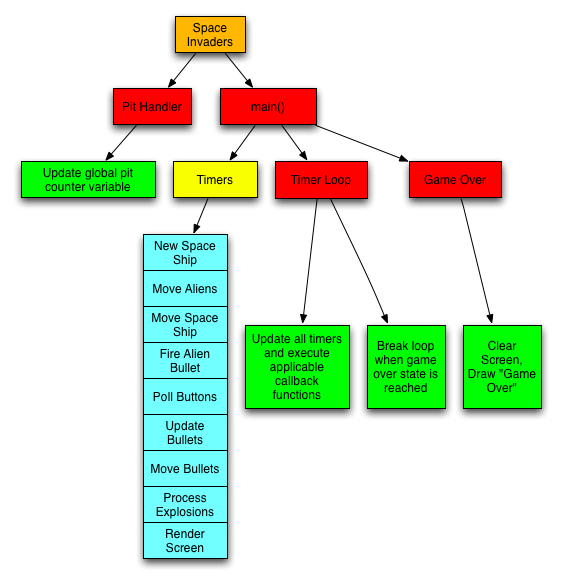
\includegraphics[scale=.80]{Space_Invaders_Overview.jpg}
\caption{Space Invaders Overview. The red blocks represent the functions that form the skeleton of the program. The green blocks represent the actions are are performed in those function. The yellow block represents the global array of implemented timers. The blue blocks represent the individual timers used to update the state of the game, or render the screen.}
\label{fig:overview}
\end{figure}

\subsubsection{Timers}
\label{sec:timers}
The sequence of events in the Space Invaders game is controlled using timers. After initializing the state of the game and creating timers, main() enters an infinite loop, determining when timer functions should be called. A timer is a structure that contains the interval of ticks between calling its registered callback function. Each time the PIT timer interrupt invokes the PIT handler, the global variable pit\_counter is incremented. Because of the complexity of the game, many timers currently exist. These include:

\begin{itemize}
\item \textbf{New Space Ship:} If the mothership is not currently on the screen, this timed event has a random probability of initializing the mothership on the screen.
\item  \textbf{Move Aliens:}  Moves all the aliens by a configurable amount of pixels.  If the aliens reach the bottom of the screen, the Game Over state is initialized.
\item  \textbf{Move Space Ship:}  If the mothership is currently on the screen, it moves by a configurable amounts of pixels across the screen.
\item  \textbf{Fire Alien Bullet:}  If less than four alien bullets are currently on the screen, this timed event has a random probability of initializing a new alien bullet on the screen.  A random, non-empty column among the aliens is chosen, and the bullet is fired from the lowest alien in that column.
\item  \textbf{Poll Buttons:}  Checks the value of the push buttons.  If the left button is pushed, the tank move  left by a configurable amount of pixels.  If the tank is already on the left edge of the screen, nothing is performed.  If the right button is pushed, the tank moves right by the same amount.  If the tank is already on the right edge of the screen, nothing is performed.  If the middle button is pushed, a new tank bullet is fired from the tank.  If there is already a bullet on the screen, nothing is performed.
\item  \textbf{Move Bullets:}  All bullets move across the screen by their configured amount of pixels.  Alien bullets move down the screen and tank bullets move up the screen.  The location of each bullet is checked to detect possible collisions.  See the section \textit{Detecting Collisions} for more details.
\item  \textbf{Update Bullets:}  Updates the stage of animation for each active alien bullet as they move across the screen.
\item  \textbf{Process Explosions:}  Three types of explosions exist that exhibit different behavior.  This timer function updates the animation of the explosion. When the animation sequence is fully performed, it is no longer drawn to the screen.
\item  \textbf{Render Screen:}  Renders the screen.  See the section \textit{Rendering} for further details.
\end{itemize}

A PIT handler is used to increment the global variable pit\_counter.  After initializing the state of the game and creating timers, main() enters an infinite loop that performs the following:
\begin{enumerate}
\item{} A snapshot of pit\_counter is taken.  
\item{} This value is compared with the value of the previous snapshot.
\item{} It iterates through each timer and increments the timer's counter.
\item{} If the timer's counter exceeds the maximum value, it resets the counter and executes the timer's registered callback function.
\end{enumerate}

The timer loop will continue to run until the game over state is reached.

\subsubsection{Detecting Collisions}
Figure~\ref{fig:collisions} demonstrates the general logic used to determine a collision. Each time a bullet moves, its coordinates are compared against the coordinates of the bunkers, tank, aliens, and mothership. The collision detection algorithms are implemented in the detectCollision() function.
 
If the bullet is a tank bullet, its coordinates are compared against the coordinates of the bunkers, aliens, or mothership. The different collision scenarios are as follows:

\begin{itemize}
\item If it is within the coordinates of the bunkers, the collision detection function determines which bunker, and bunker block it hit. If the block is still active, the bunker is eroded and the bullet is deactivated.
\item If it is within the coordinates of the aliens, the alien row and column are determined to specify the hit alien. If the alien is still active, the type of alien is determined. If the bullet is within the the bounds of that alien type, they alien explodes and the bullet is deactivated.
\item If it is within the coordinates of the mothership, the mothership explodes and the bullet is deactivated.
\end{itemize}

If the bullet is an alien bullet, its coordinates are compared against the coordinates of the bunker, and tank.

\begin{itemize}
\item If it is within the coordinates of the bunkers, the collision detection function determines which bunker, and bunker block it hit. If the block is still active, the bunker is eroded and the bullet is deactivated.
\item If it is within the coordinates of the tank, the tank explodes, and the bullet is deactivated.
\end{itemize}

\begin{figure}[H]
\centering
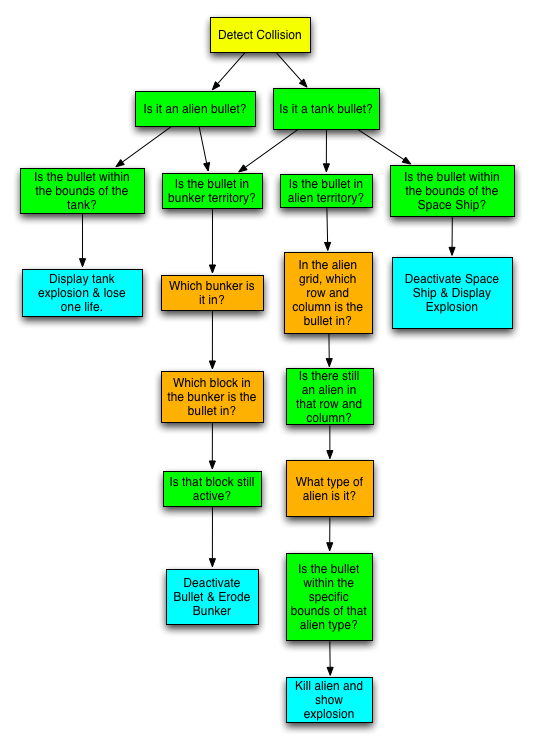
\includegraphics[scale=.7]{Detect_Collision.jpg}
\caption{Collision Detection. The green blocks represent the state that must be met to continue. The orange blocks represent the process of determining the specific object that was hit. The blue blocks represent the actions taken to change the game state during a collision.}
\label{fig:collisions}
\end{figure}

\subsubsection{Rendering}
The screen is rendered on regular intervals by using a timer. The rendering process occurs whether or not the the state of the game is changed. This mirrors the rendering process of the flash game. This rendering process creates a very smooth animation process.


\subsubsection{Double Buffering}
Flickering on the screen is caused by drawing and erasing objects on the same screen. In order to avoid flickering, double buffering is used. Double buffering involves writing to another part of memory, or frame than the currently displayed screen. The currently displayed frame is never modified.  After drawing is finished on this separate frame, the program changes the screen to display this new frame. Thus, all modifications to the screen occur on an inactive frame. Figure~\ref{fig:render} shows the steps in rendering process.

\begin{figure}[H]
\centering
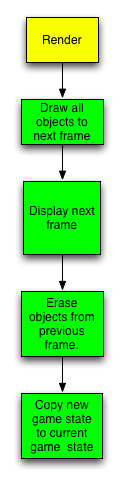
\includegraphics[scale=.8]{Render.jpg}
\caption{Double Buffer. The currently displayed frame is never modified. Only after writing correct values to a new frame, the program changes the screen to display it.}
\label{fig:render}
\end{figure}

\subsubsection{Flying over the bunkers}
Aliens must march over bunkers when they reach them. However, erasing and redrawing the aliens can erase blocks of bunkers, even though they aren't inactive. In order to redraw the bunkers properly, the state of the bunkers are always drawn in a dedicated frame, FRAME3.  As an alien is erased, the program accesses the bunker pixel values that are stored in this frame to restore these pixels. When an alien is drawn in the bunker region, the background values of BLACK are replaced by the values stored in FRAME3. Thus the alien appears to march over the bunkers.


\subsection{Software APIs}
\subsubsection{Game State}
Because our engine implements passive rendering (i.e. the screen is rendered whether or not the game state has changed), most of the game logic involves modifying the game state.  There are two copies of the game state at any given point in time.  The current state reflects what is currently drawn to the screen.  All modification are made to the next state of the game.  When the screen is rendered, the next state is copied to the current state.

To facilitate testing and to protect our global variables, most of our game logic exists in pure functions.  They will accept the data as parameters and return a copy of the data.

Example:

new\_tank\_bullet = moveBullet(new\_tank\_bullet);

This will take the current coordinates of the tank bullet, and increment the y coordinate (causing the bullet to move up).  The bullet struct is not modified by the function call, but instead a new bullet is returned.  The global new\_tank\_bullet is assigned to the returned value.  The following functions act in a similar manner:

\begin{itemize}
	\item Bullets:
		\begin{verbatim}
		bullet moveBullet(bullet new_bullet);
		bullet updateBullet(bullet new_bullet);
		\end{verbatim}
	\item	Coordinate Objects (such as aliens, space ships or the tank):
		\begin{verbatim}
		coord_object moveRight(coord_object aliens);
		coord_object moveLeft(coord_object aliens);
		coord_object moveDown(coord_object aliens);
		coord_object moveAliens(coord_object new_aliens_coord, int * aliens);
		coord_object moveShip(coord_object ship);
		\end{verbatim}
		\textbf{Note:}  Some functions take additional game state parameters, such as moveAliens, which influence the behavior of the function.  These are not modified in any way.
	\item Explosions:
		\begin{verbatim}
			explosion updateExplosion(explosion new_explosion);
			explosion newExplosion(explosion temp_explosion, int x, int y);
			explosion newShipExplosion(explosion temp_explosion, int x, int y);
		\end{verbatim}
	\item There are also methods that deal with interaction of multiple object types:
		\begin{verbatim}
			bullet fireAlienBullet(coord_object new_aliens_coord, int row, int col);;
			bullet fireBullet(coord_object tank);
		\end{verbatim}
	\item Another class of methods are those dealing with multiple parts of the game state:
		\begin{itemize}
			\item
			\begin{verbatim}
			bullet detectCollision(bullet new_bullet);
			\end{verbatim}

			  This method takes a bullet as a parameter.  It compares the coordinates of the bullet to the location of the bunkers, the aliens, and the tank.  If it is determined to be a hit, the method will deactivate the bullet and either erode a bunker or explode an alien, depending on what sort of collision was detected.  It then returns the updated bullet.  While it doesn't modify the bullet, this is not a pure function because it does modify other aspects of the game state (eroding bunkers, killing aliens, or losing lives).
		\end{itemize}
\end{itemize}

If the functions listed above are the building blocks of the application, then the glue consists of the callback functions of the Timers.  (See Section~\ref{sec:timers} under Timers)  The callback functions modify the game state through all of the above functions.  

\subsubsection{Rendering of images}
Images are stored in memory as an encoded bitstring.  A Xuint16 can represent a single line of an image up to 16 pixels wide.  Each image is an array of these encoded bitstrings.  To draw to the screen, the images are scaled up to double their size.  A single pixel in the stored image corresponds to a 2 by 2 block of pixels on the screen. Each image type has it's own rendering function.  The functions typically take an x and y coordinate, a frame to draw to, and a color to draw.  To erase, the functions draw black to the screen.  In some situations, such as around the bunkers, the functions read from a third frame of the screen in order to erase to a non-black value.  This is very costly to performance, so this is only done in necessary regions of the screen.  

Because we use passive rendering, the only function that modifies the screen is our render function.  This is called by a Timer and is by default called twenty times a second.  No other functions will call render.  Render calls draw and erase function for each object on the screen.

\subsection{Meeting the Game Specifications}

\subsubsection{The Tank}
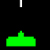
\includegraphics[]{tank.jpg}

The buttons are polled in regular intervals using the the Poll Buttons timer. As the tank moves laterally, it is drawn to a new frame, in a new position. The screen switches to that frame, and the tank in the old frame is erased, creating a smooth animation. Furthermore, the tank can only move to the edge of the screen. When it reaches the edge of the screen, it stops, unable to move left. Each time the tank moves, its coordinates are compared against the edges of the screen. When it reaches the edge of the screen, the moveTank() function doesn't change the coordinate of the tank.

The user is able to hold down the left or right buttons to keep the tank moving across the screen. This is done by using a timer to control the speed of the tank movement. The Poll Buttons timer is checked in regular intervals. If a left or right button is asserted, it is update the location of the tank, moving left or right.

When an alien bullet hits the tank, the tank explodes. This is implemented using three tank animations that are stored in an array. Each time the explosion update timer is called, the animation changes to a new position in the array. This happens on regular intervals when an explosion occurs. The tank appears to explode because of the implemented double buffering and switching between these items in the array. A new animation is drawn to the new frame, while the old animation in the old frame is erased.

Each time a tank explodes, the lives global variable is decremented and one tank is erased from the screen on the top right corner.

\subsubsection{Mothership}

\includegraphics[]{big-alien.png}

The mothership is randomly activated on regular intervals, flying from left to right. This means that after a certain period of time, the program determines whether or not the mothership should appear. The probability of its appearance is configurable.

When the mothership explodes, a random integer between 50 and 350 flashes for one second in its place. This score is added to the total score and displayed in the top left corner of the screen. The flashing is done by alternating between two animations in regular intervals. One animation shows the score of the hit, and the other animation displays black. Thus the score appears to flash.

\subsubsection{Aliens}

\includegraphics[]{aliens.jpg}

There are 55 aliens total that are formed in an 11 by 5 grid. Each alien is drawn in a 30 by 30 pixel block. Only the coordinates of the top left corner of the top left alien is stored. All other aliens reference this value. An array 55 integers is kept globally to store whether or not the alien is active. Only aliens that are active are redrawn to the screen. The first two rows of are the widest aliens, the next two rows are a little narrower and the top row has the narrowest alien.

An alien becomes inactive when a bullet hits it. A hit occurs when at least one of the pixels of the bullet overlap the pixels of an alien. Each row of aliens is different. Although the aliens are drawn in blocks, unless the bullet overlaps a white pixel of an alien, it will not explode. This is necessary for a bullet to fly between aliens. For example, a bullet can miss a bottom row alien, and hit a second row alien. When an alien is killed, an explosion replaces it for a short time before dissipating. The other aliens continue onward while the explosion occurs.

Aliens march over bunkers when they reach them. However, erasing and redrawing the aliens can erase blocks of bunkers, even though they aren't inactive. In order to redraw the bunkers properly, the state of the bunkers are always drawn in a dedicated frame, FRAME3.  As an alien is erased, the program accesses the bunker pixel values that are stored in this frame to restore these pixels. When an alien is drawn in the bunker region, the background values of BLACK are replaced by the values stored in FRAME3. Thus the alien appears to march over the bunkers.

The aliens move laterally in increments of 4 pixels.  When the rightmost aliens reach the right edge of the screen, the grid of aliens move down 7 pixels and start moving left.  When the leftmost aliens reach the left edge of the screen, they move down 7 pixels and start moving right.  The rightmost alien and leftmost alien is the closest alien to the respective sides that has not been killed. This means that when the rightmost column of aliens are destroyed, the aliens march toward the side of the screen until the next column hits that side. The aliens continue this pattern of movement until the bottommost row of alive aliens reaches the bottom of the screen. 

We check for the rightmost or leftmost active alien by iterating each alien in each column. If there isn't an active alien in a column, the next inner column is checked until an active alien is discovered. When we move the aliens, we do not change the direction of the grid of aliens until the rightmost or leftmost alien reaches the edge of the screen.

Each time an alien is killed, the animation speed of the aliens increases logarithmically. This is done using the timers. Each time an alien is destroyed, the time between alien movements decreases by 10%. This means that when there is only one alien, it will move 10 times as fast as when it started.

\subsubsection{Scoring}
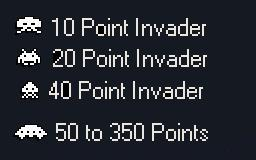
\includegraphics[]{scoring.jpg}

Points are earned when the mothership is destroyed, or an alien is killed. This happens when at least one pixel of bullet overlaps a drawn pixel of an alien or mothership. The lower two rows of aliens, middle two rows of aliens, and the top row of aliens are worth 10, 20 points and 40 points per alien, respectively. When the mothership is destroyed, a value between 50 to 350 points is added to the total score.

The score is displayed in the top left corner of the screen. All numbers are left justified, imitating the flash game. Commas are drawn slightly lower than numbers. Thus, they appear to be in the correct position.


\subsubsection{Tank Bullets}
Tank bullets are fired when the middle button is pushed. The Poll Buttons timer checks the middle button on regular intervals for changes. When it detects that the middle button has been pushed, a bullet is drawn to the screen just above the center of the tank, and the global tank bullet variable is set to active. This is done by checking both the middle, left and right buttons every time the buttons are polled. Each button handler changes the state of the game before the next render. Thus the tank can move, change directions and fire between two calls to render(). Then, on regular intervals, the bullet moves upward until it leaves the screen or hits the mothership or an alien. When it strikes any of these two objects, it is deactivated, and it is neither drawn to the screen or move. Explosion sequences are activated when the tank bullet hits them.

When a bullet is on the screen, more tank bullets are not created until the middle button is pushed again, and the tank bullet is off the screen.  Each bullet travels at a configurable rate.

\subsubsection{Alien Bullets}
There are two types of alien bullets:
\begin{enumerate}
\item{}  Zig zag bullets rotate cyclically through the following appearances:

\begin{enumerate}
\item 
 
\includegraphics[scale=2]{ZigBullet0.png}
\item 
 
\includegraphics[scale=2]{ZigBullet1.png}
\item
 
\includegraphics[scale=2]{ZigBullet2.png}
\item
 
\includegraphics[scale=2]{ZigBullet3.png}
\end{enumerate}

\item{}  Cross bullets oscillate through the following appearance:

\begin{enumerate}
\item
 
\includegraphics[scale=2]{TBullet0.png}
\item
 
\includegraphics[scale=2]{TBullet1.png}
\item
 
\includegraphics[scale=2]{TBullet2.png}
\end{enumerate}

\end{enumerate}

Each of these animation sequences are stored in an array of encoded bits. The location of the bullet determines which animation is drawn to the screen using modulus. Thus, as the alien bullets move downward, they cycle through the animations, making them appear to zig zag or oscillate.


The bullet regularly moves using a timer by a configurable amount of pixels. Each time the timer calls the moveAliens() callback function, the bullets position is updated, and compared with the position of the bunkers and tanks. If any of the bullet's pixels overlap any of the pixels in these objects, an explosion occurs, and the bullet is deactivated.

Each bullet is ejected from the center of an alien, randomly chosen to be the bottommost alien of an active column. This means that when a bottom row alien is destroyed, the alien just above it is able to fire a bullet. We implemented this by randomly choosing a column of aliens. Iterating upward, we searched for the first active alien in that column. When it was found, the alien bullet used the coordinates determine where to be drawn..

Only 4 alien bullets are active at a time. In our code, this means that there are only 4 alien bullet structures. Once a bullet is active, it cannot be reactivated until it strikes a bunker or tank, or leaves the screen. The movement of the alien bullet determines if it destroyed an object. If its new coordinates cause it to overlap an active bunker block or tank, it causes them to erode or explode.

No black boxes surround the alien bullets. In other words, when it leaves an alien, or strikes an object, an overlay of a black box cannot be seen. This is done by Only drawing only the foreground color of the bullets.

\subsection{The Bunkers}

When a tank or alien bullet strikes a bunker, the bunker erodes. This is done by dividing the bunker into 12 equal size blocks. An array of 48 integers controls the state of each block. When a block is hit by a bullet, it's associated integer is incremented until it reaches 4. When it reaches this state, bullets can pass through them, and are not destroyed when they hit them.

A function strategically places the bunker block in the correct positions of the screen. Since they do not move, they are always drawn in the same position.

\subsection{End of Game}
The game ends when one of the following three events occur:
\begin{enumerate}
\item The bottommost row of aliens that are alive reach the bottom of the bunkers.
\item The tank has been destroyed three times.
\item All aliens are destroyed.
\end{enumerate}
When the game ends, a game over screen is displayed.

First, when the aliens move, if their position is is equal to the position of the bottom of the bunkers the game\_over global variable is set to 1. Second, when the tank is destroyed, if no other lives exist, the game\_over global variable is set to 1. Third, when an alien is destroyed, if not other aliens are active, the game\_over global variable is set to 1.

In the main() function, when the game\_over global variable is set to 1, it stops checking the timer values and jumps out of the while() loop. The aliens are erased, and  the game freezes with a large GAME OVER text in the center of the screen.

\subsection{Appearance}
The game appearance is identical to the flash version of Space Invasion. The game runs smoothly and at a decent speed. The screen is also updated close to the same rate as the flash-based game. No artifacts appear on the screen. No flickering occurs on the screen.

The render() function makes this possible. Because the screen is updated on small intervals, the screen is consistently updated close to the rate of the flash-based game. This eliminates flickering, making the animation smooth.

\chapter{Game Audio}
\section{AC97 Operation}
\subsection{ Loading Audio Files From the Compact Flash}
To copy the data from the compact flash to the DDR, the following steps are taken:
\begin{enumerate}
\item Read from compact flash to temp space
\item Using wav\_header struct, extract necessary header information
\item Preprocess wav file for FIFO buffering
\item store in DDR, store address and header in sound struct
\end{enumerate}

\subsubsection{Reading from Compact Flash}

We use given function sysace\_fread() to retrieve the sound data from the compact flash card. The data is read one byte at a time, and placed in a designated, tempSpace address in memory on the DDR. 

\subsubsection{Wav Sound Struct}

Once the file is in the DDR memory (at the tempSpace address), A wave struct is overlayed on the memory address. This allows us to parse out the individual attributes in the header. The values that are useful are the sample rate, the file size, bits per sample, and the number of channels. 

\subsubsection{Preprocess Wav File for FIFO Buffering}

Because there is no live mixing of sounds, we can preprocess the wav sound data before storing the data permanently in DDR memory. This means that we can avoid processing the sound during game play, speeding up our implementation. If we were to mix sounds, we could not do this. We would have to store the raw data, and process on the fly, adding additional sounds. 

The FIFO expects a 32 bit integer of sampled sound data. The upper 16 bits represent the right channel, and the lower 16 bits represent the left channel. Because the data is stored in the DDR memory as 8 bit characters, they need to be cast into integers, and placed in both the upper and lower 16 bits of the integer respectively.  We also amplify each channel by shifting the value 8 bits to the left, effectively multiplying each value by 256. This increases the volume to reasonable levels.

\subsubsection{Store sound file in memory}

In order to keep track of multiple sound files, we have an array of our sound struct in global memory.  The array contains information about the file, such as sample rate and length, as well as a pointer to the sound data in memory.

The sound data is stored on the DDR.  We have a set starting address for the first sound.  The starting address for the sound is stored in its struct along with its length and other data.  The next sound is stored directly following it in memory.  We dynamically adjust the starting address for each new sound as it is parsed in.

In order to keep tract of individual sounds, we use an enum variable to index into our sound struct array by a descriptive name.  (i.e. sounds[TankExplode] is the struct for the tank explosion sound)

\subsection{AC97 Operation}

In order to use the AC97 properly, multiple components of the system are used.  Most of the complexity in the system is based around the interrupt based model of keeping the AC97 Controller FIFO filled. As shown in Figure~\ref{fig:AC97}, the PowerPC is responsible for this activity, and must enable its non-critical exceptions in order to accept interrupts from the OPB Interrupt Controller. The OPB Interrupt controller is responsible for accepting interrupts from the OPB\_AC97 Controller when the FIFO is less than 50% full. As long as the FIFO does not overflow or underflow, the signals sent to the AC97 hardware (and thus the speakers) is clean, free of clicking.

\begin{figure}[H]
\centering
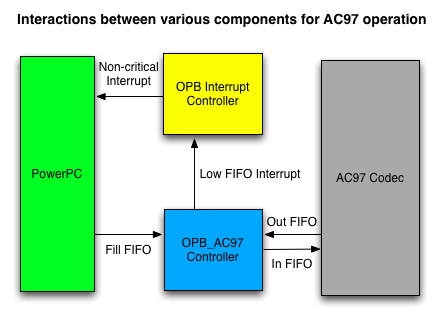
\includegraphics[scale=.7]{AC97_Operation.jpg}
\caption{AC\_97 Operation. The OPB\_AC97 Controller sends a signal to the OPB Interrupt Controller when its FIFO is less than 50\% full. The OPB Interrupt Controller interrupts the PowerPC, which sends data to the OPB\_AC97 Controller FIFO.}
\label{fig:AC97}
\end{figure}

\subsubsection{PowerPC}

The PowerPC is responsible for keeping the AC97 Controller FIFO filled.  When the FIFO level is low (less than 50%), it sends and interrupt.  The PowerPC needs to accept the interrupt and respond by adding data to the AC97 Controller FIFO.  In order to do this, the PowerPC must be configured to respond to interrupts.  The exception handler must be configured to allow non-critical interrupts.  Once an interrupt is received, it should call XIntc_InterruptHandler, which is configured by the OPB Interrupt Controller.

\subsubsection{OPB\_AC97 Controller}

The OPB\_AC97 Controller is responsible for managing its FIFO of data.  This data is sent serially to the AC97 codec at the configured sample rate.  When the FIFO level is low (below 50%) the OPB\_AC97 Controller sends an interrupt via the OPB Interrupt Controller.  This interrupt is handled to fill the FIFO with data. However, if the PowerPC overfills the FIFO, data is lost, and the signal to the AC97, and thus the speaker is not clean. Also, if the FIFO is empty, it will continue to play from the top of the FIFO. This can result in clicking sound. Care is taken to to underflow or overflow the FIFO. The OPB\_AC97 Controller's interrupt mechanism must be enabled before it sends any interrupt signals.

\subsubsection{OPB Interrupt Controller}

The OPB Interrupt Controller receives interrupts from various pieces of hardware.  In our case, it receives interrupts from the OPB\_AC97 Controller.  Each interrupt type is configured to be handled by individual handlers.  This configuration takes place in the OPB Interrupt Controller. A wrapper is provided to handle the setting of the handler functions. This wrapper also allows easy initialization of the OPB Interrupt Controller.

\subsubsection{AC97}

The AC97 is hardware that is connected to a speaker. It receives data from the FIFO in the OPB\_AC97 Controller. Because the AC97 requires analog signals, the OPB\_AC97 Controller converts the digital signals in its FIFO to analog before sending it to the AC97 hardware. The AC97 doesn't concern itself with the sample rate, but only plays the signals that it receives from the controller.

\subsection{Sound Triggering}

\subsubsection{Playing a sound}
In order to facilitate an interrupt driven model, we have a global pointer to a Sound struct  called current\_sound.  The interrupt handler will fill the FIFO with data from the current sound.  The position within the sound is stored in the struct so the interrupt handler can continue where it left off.  With this structure, we need only set current\_sound to the address of the sound struct we would like to play.  If current\_sound is not assigned or is null, the FIFO is filled with silence.

\subsubsection{Our sounds}

Because we are only playing one sound at a time, we have a priority among sounds which determines whether or not a sound can interrupt the one currently playing.

We have the following sounds in our game, from lowest priority to highest priority:

\begin{itemize}
\item Alien Movement - The four sounds determining alien movement play cyclically.  The sound played is determined by the position on the screen and its direction of movement.  This results in sounds playing in the proper order even as the aliens reach an edge and change direction.  This sound is interrupted by all other sounds.  Unless interrupted, it will play until it finishes
\item Tank Bullet - When a bullet is fired from the tank, it makes a sound.  It will interrupt the Alien Movement sounds, but will be interrupted by Space Ship Movement, Space Ship Explosion, and Tank Explosion.  Unless interrupted, it will play until it finishes.
\item Space Ship Movement - When the Space Ship enters the screen, this sound is played.  When it leaves the screen, the sound is stopped.  It will only be interrupted by Space Ship Explosion and Tank Explosion.
\item Space Ship Explosion - When the Space Ship is hit by a tank bullet, this sound is played while the score value flashes.  It is interrupted only by the Tank Explosion.  Unless interrupted, it will play until it finishes.
\item Tank Explosion - When the tank is hit by an alien bullet, this sound is played.  It is never interrupted and will continue to play until finished.
\end{itemize}

In our code we wrote a nice wrapper for playing and stopping sounds.  One need only make a call to playSound( Sound * new\_sound ).  It takes as its parameter the address of the Sound struct to be played.  If the currently playing sound is higher priority than the one passed in, it will not be played.  Otherwise, the currently playing sound is stopped and the new sound is played.  The sound that was interrupted is reset so that it begins from the beginning the next time it is played.  The current sound can be stopped with a call to endSound(Sound * sound).  It takes the address of the Sound struct to be stopped.  This will result in silence being played until a new sound has been played.



\chapter{Bug Reports and File Organization}

\section{Bug Reports}

\subsection{Drawing Bullets}
During our design phase, we found a bug involving the drawing of alien bullets to the screen. 

First, we had difficulty cycling through the different different stages of the bullet. We were able to cycle through four stages, however, the fourth state was a different bullet type entirely. We fixed the bug by placing a simple if statement in our draw bullet loop. When the bullet was in the fourth stage, it cycled back to the third state to and reset its state to the first state. In this way we were able to use the same functions for a four cycle bullet and a three cycle bullet.

Second, we found a bug when the first bullet was fired. Without permission, another bullet was drawn at pixel location (0,0). We found the problem by analyzing our bullet structs. We discovered that our bullet variables were not initialized to zero. We assumed that they would be initialized to zero, but a random value was placed there. When we initialized all variables, the bug was fixed.

\subsection{Destroying Aliens}
During our design phase, we found a bug involving the destroying of aliens. We thought that the lab instructions said to give find a random number between 0 and 54 and destroy that alien. When we tried to pass it off, the TA told us that we needed to ask the user to input a number. To fix the bug, we used the read() function to acquire a number from the user, one integer at a time. We destroyed the alien that corresponded to that number.

\subsection{Moving Aliens to Right of Screen}
We initially had some naive logic concerning the aliens reaching the edge of the screen.  We set a hard limit for the grid of aliens.  Once the top left corner of the grid had reached the limit, the aliens moved down and changed directions.  This did not account for all aliens on the edge of the grid being dead, which would require the alien grid to move one column closer to the edge than it did with all aliens alive.  We fixed this by using a more dynamic approach.

\subsection{Overlay of Bullet Black Boxes}
During our design phase, we found a bug involving the overlay of the bullet black boxes. We discovered that as a bullet was launched, and flew over objects on the screen, it had black boxes surrounding it. We have not yet resolved this bug, but will do so in the near future.

\subsection{One Alien Firing Two Bullets Simultaneously}
While trying test our implementation of aliens firing bullets, we encountered a situation in which an alien fires two bullets on top of each other.  They will appear as one bullet.  We solved this by limiting the firing of a bullet until the first one has moved out of its original position. 

\subsection{Overwriting Memory}
With good intent, we wrote a for loop to iterate through an array, and ended it using a call to sizeof() in our main() function. Our screen exhibited strange behavior, drawing objects in the top left corner of the screen. Ensuring that we initialized our objects to be inactive, they still appeared there. Using print statements throughout the program, we determined that the initial values of our variables were incorrect. They seemed to change value within only a small block of initialization code in main(). Determined to discover the issue, we closely scrutinized our code and discovered the issue. We learned that sizeof() returns the number of bytes of the entire array, instead of the number of objects in the array. After correcting this mistake, our issue was resolved.


\subsection{Tank Out of Bounds}
During most of our initial tests, we did not try to push the tank to the edge of the screen. After accidentally holding down the right button, we discovered that part of our tank disappeared into the side of the screen. To fix this issue, we inserted an if statement to check the position of the tank every time it moved. If it is within a given range of the left or right side of the screen, it is unable to move past that point. However, it is still able to move the opposite direction.

\subsection{Not Enough Bunker Blocks}
After constructing the bunkers using the bunker block images, we discovered that a systematic comparison with the position of the blocks with the bullet positions was not possible. We had only used 10 blocks per bunker, but we needed 12. The two blocks in the bottom and center of each bunker needed to be constructed and placed there. We added 8 new places in the global bunker block state array for each of these new blocks and set each state to 4. Therefore, when a bullet hit them, they were already considered destroyed, and the bullets flew through them. This greatly simplified our code.

\subsection{Tank Movement During Explosion}
Alien bullets are capable of destroying a tank. When a tank is destroyed, it is supposed to flip through a series of animations to appear to explode. It soon became evident that as the tank exploded, it was capable of moving during the explosion. The solution was simple. When the moveTank() function is called, it now determines if the tank is currently exploding. If it is, it does not update its position, but simply returns. The tank now appears to be frozen while it explodes.

\subsection{Tank Bullet Grazing Aliens}
After playing the game several times, it became clear that if a bullet overlapped an alien by only 2 pixels, it did not explode. After doing some investigation, it became clear that when the bullet moved, the function that compares the bullet position and the alien position was off by 2 pixels. with a simple addition of 2, the alien now explodes when the bullet's pixels overlap any of the aliens' pixels.

\subsection{Knowing when a sound has finished playing}
We had some trouble determining from our interrupt handler when a sound was finished playing.  We were depending upon a return value for our method that fills the FIFO with sound data, but were getting unexpected results.  It turned out that we had set the return type to void instead of int and when we fixed it all was working great!

\subsection{AC97 Interrupts}
When we were implementing our interrupt driven sounds, we followed the wrapper documentation to determine how to play sounds. We believed that we had retrieved all of the function calls that were necessary, however, we were missing a few. We had not enabled the interrupts on the AC97 controller. Once we did that, we received the expected interrupts.

\subsection{Big Endian}
When we attempted to parse our wav file for the sample rate, it appeared that we were correctly playing the sound with the correct sample rate. However, we found that the sound was being played much too fast. One error was that we were not setting the sample rate every time and was hard coded to 44kHz. Another issue had to do with how the data was read from the compact flash drive. The compact flash drive is setup in little endian, however the function to read from the flash drive expects big endian. Thus, the bytes were swapped. After we correctly swapped the bytes back, we were able to place the correct sample rate into the AC97 and play our sound.

\subsection{Initial Failure}
When we first began implementing sound, our experiments were erratic. We attempted to perform all of our parsing, and playing simultaneously in the main() function. It turned into spaghetti code, and was very disorderly. After several hours of looking through the code, we could not determine why the sound from the AC97 was scratchy. We separated our code into multiple functions, and found it much easier to implement the sound. The bugs became more clear, and we were able to finish the lab code only a few hours later.

\end{document}
